% Standalone source: compile twice with pdfLaTeX; no external files required.
\documentclass[10pt,letterpaper]{article}
\usepackage[T1]{fontenc}
\usepackage[utf8]{inputenc}
\usepackage{lmodern}
\usepackage[hmargin=0.8in,vmargin=0.7in]{geometry}
\usepackage{amsmath,booktabs,array,float,graphicx}
\usepackage{placeins}
\usepackage[font=small,labelfont=bf,skip=4pt]{caption}
\captionsetup[figure]{skip=6pt}
\usepackage{enumitem}
\setlist[itemize,enumerate]{topsep=2pt,itemsep=1pt,parsep=0pt,partopsep=0pt}
\usepackage[hidelinks]{hyperref}
\hypersetup{
 pdftitle={Training a neural network surrogate for nonlinear CGYRO nuclear fusion simulations via existing quasilinear TGLF simulations},
 pdfauthor={Sweekrit Bhatnagar, Ryan Lindberg, Joseph Calderon, Aryan Nath, Emily Belli, Jeff Candy, Igor Sfiligoi},
 pdfsubject={UC San Diego DSC 180 Quarter 2 research proposal}
}
\setlength{\parindent}{0pt}
\setlength{\parskip}{6pt plus 2pt minus 1pt}
\setlength{\emergencystretch}{1em}
\makeatletter
\renewcommand{\section}{\@startsection{section}{1}{0pt}
 {14pt plus 2pt minus 2pt}{5pt}{\normalfont\large\bfseries}}
\makeatother
\pagestyle{plain}

% ---- Table conventions (all tables: \small, caption above, never split, placed where they appear in the source) ----
\setlength{\textfloatsep}{12pt plus 2pt minus 2pt}
\setlength{\intextsep}{10pt plus 2pt minus 2pt}
\newcolumntype{L}[1]{>{\raggedright\arraybackslash}p{#1}}
\newcolumntype{B}[1]{>{\raggedright\arraybackslash\bfseries}p{#1}}
% \opt starts one bullet inside a table cell; wrapped lines align with the text.
\newcommand{\opt}{\par\hangindent=0.75em\hangafter=1\noindent\textbullet~}
% \q adds an italic note under a row name.
\newcommand{\q}[1]{\par{\normalfont\itshape #1}}
% \rowsep ends a row and draws a thin rule between rows.
\newcommand{\rowsep}{\\ \specialrule{0.4pt}{4pt}{4pt}}
% \tablestyle sets the shared font, row height, and paragraph spacing inside tables.
\newcommand{\tablestyle}{\small\renewcommand{\arraystretch}{1.15}\setlength{\parskip}{0pt}}

\begin{document}
% ---- Title block ----
{\centering\setlength{\parskip}{0pt}
      {\fontsize{14}{17}\selectfont\bfseries
            Training a neural network surrogate for nonlinear CGYRO\\
            nuclear fusion simulations via existing quasilinear TGLF simulations\par}
      \vspace{8pt}
      Sweekrit Bhatnagar$^{1}$, Ryan Lindberg$^{1}$, Joseph Calderon$^{1}$, Aryan Nath$^{1}$\par
      \vspace{2pt}
      Mentors: Emily Belli$^{2}$, Jeff Candy$^{2}$, Igor Sfiligoi$^{3}$\par
      \vspace{4pt}
      {\small\itshape
            $^{1}$Hal\i c\i o\u{g}lu Data Science Institute, UC San Diego \enspace
            $^{2}$General Atomics \enspace
            $^{3}$San Diego Supercomputer Center\par}
      \vspace{6pt}
      DSC 180 \enspace $\cdot$ \enspace Quarter 2 Research Proposal\par
}
\vspace{2pt}

\section{Objective}

Use broad TGLF data and sparse nonlinear CGYRO references to train a neural network (NN) correction to TGLF for heat and particle transport, and test whether it moves predictions closer to CGYRO across plasma regimes.

\section{Background: gyrokinetic simulation and quasilinear models}
\label{sec:background}

Turbulence driven by temperature and density gradients dominates heat and particle losses from the core of a tokamak. Transport codes predict plasma profiles by repeatedly asking a turbulence model for the fluxes produced by local plasma parameters $x$: gradients, temperature and density ratios, magnetic geometry, collisionality, and rotation. We predict three fluxes in gyro-Bohm units: the ion heat flux $Q_i$, the electron heat flux $Q_e$, and the electron particle flux $\Gamma_e$.

\textbf{CGYRO (nonlinear gyrokinetics)} \cite{candy2016} is the high-fidelity reference for turbulent transport.
\begin{itemize}
      \item \textbf{Physics model:} gyrokinetics averages over the fast gyration of particles around magnetic field lines, reducing six phase-space dimensions to five while keeping the physics that drives turbulence.
      \item \textbf{Method:} CGYRO solves the nonlinear gyrokinetic equations for each species in a local flux tube, runs until the turbulence saturates, and time-averages the fluxes.
      \item \textbf{Cost and noise:} one run costs thousands to hundreds of thousands of CPU-hours, and the averaged fluxes carry statistical noise.
      \item \textbf{Linear runs:} much cheaper, but they give only growth rates, not the saturated turbulence level.
\end{itemize}

\textbf{TGLF (quasilinear model)} \cite{staebler2007} approximates gyrokinetics in three steps:
\begin{enumerate}
      \item \textbf{Linear stability:} a reduced gyro-Landau-fluid model gives, at each wavenumber $k_y$ from ion to electron scales, each unstable mode's growth rate $\gamma$, its frequency $\omega$ (which identifies the instability type), and its quasilinear weight (flux per unit fluctuation amplitude).
      \item \textbf{Saturation:} a rule calibrated against nonlinear simulations estimates the saturated amplitude at each $k_y$.
      \item \textbf{Flux:} the predicted flux is the sum over $k_y$ of weight times amplitude.
\end{enumerate}

A TGLF call takes seconds to minutes, and NN surrogates of TGLF are faster still \cite{meneghini2017}.

\textbf{Where TGLF and CGYRO disagree.} TGLF's linear step tracks linear gyrokinetics reasonably well. Most of the gap to nonlinear CGYRO comes from the saturation rule, which must compress nonlinear physics, such as zonal-flow regulation near instability thresholds and coupling between ion- and electron-scale turbulence, into a formula. Successive rules, most recently SAT3 \cite{dudding2022}, have narrowed the gap but not closed it. The intermediate TGLF quantities ($\gamma$, $\omega$, quasilinear weights, and per-$k_y$ fluxes) show which instabilities drive transport, so they are useful inputs for learning where TGLF departs from CGYRO.

\section{Prior work}

Machine learning has addressed the TGLF--CGYRO gap in three ways:
\begin{itemize}
      \item \textbf{Fast TGLF surrogates:} NNs trained on TGLF reproduce its fluxes at a fraction of the cost \cite{meneghini2017}, and TGLF-WINN adds wavenumber-resolved supervision \cite{cao2026}. These surrogates inherit TGLF's errors relative to CGYRO.
      \item \textbf{Linear gyrokinetic information:} GKNN-0 uses linear CGYRO information to address differences between TGLF and gyrokinetics \cite{neiser2024}. Linear runs are cheap but miss the saturation physics behind much of the gap.
      \item \textbf{Learned saturation rules:} SAT3-NN learns saturated spectra from nonlinear CGYRO \cite{sar2026}, replacing one TGLF component with a learned one.
\end{itemize}

These studies reproduce TGLF or replace one of its components. To our knowledge, none tests whether a correction learned from a few hundred nonlinear CGYRO cases transfers to new conditions, or which TGLF information such a correction needs.

\section{Proposed work and research questions}

We test whether about 300 nonlinear CGYRO cases can support a correction to TGLF that transfers across plasma regimes. Speed is not the goal: TGLF runs for every prediction, and the aim is to get as close to CGYRO as TGLF information allows. The work has three parts:
\begin{enumerate}
      \item \textbf{Pretrained surrogate:} an NN trained on a large TGLF dataset to predict the 5th, 50th, and 95th percentiles of each flux.
      \item \textbf{TGLF-informed correction:} an NN trained on matched TGLF and CGYRO cases to predict the CGYRO--TGLF difference from TGLF fluxes, TGLF spectral features, and the surrogate's representation.
      \item \textbf{Information ablation:} a measure of how much each input contributes, compared with a surrogate-only variant that runs no physics code.
\end{enumerate}

We address four questions:
\begin{enumerate}
      \item Does the correction improve agreement with held-out CGYRO cases? By how much, in which regimes, and what causes it to fail where it makes predictions worse?
      \item Do the surrogate's 5--95\% interval width or its disagreement with TGLF predict where TGLF departs from CGYRO, and can they set how strongly to apply the correction?
      \item How many CGYRO cases does the correction need before it reliably improves predictions?
      \item Which inputs does the correction need (TGLF fluxes, spectral features, or the surrogate's representation), and how much does running TGLF add over the surrogate-only variant?
\end{enumerate}

The outcomes are an uncertainty-aware hybrid model that moves flux predictions closer to CGYRO, and evidence on where nonlinear corrections transfer and where they fail when CGYRO coverage is sparse.

\section{Data and a TGLF-informed hybrid model}

\textbf{Data.} About 300 nonlinear CGYRO cases span a range of plasma regimes. For each, we run TGLF on the same input deck, with the same version and saturation settings as the bulk data, and save both the fluxes and the wavenumber-resolved linear spectra. To pretrain the surrogate, we generate a large TGLF dataset from randomly sampled inputs at the San Diego Supercomputer Center (SDSC). We first audit all datasets for coverage, mutual compatibility, and available diagnostics. Figure~\ref{fig:pipeline} summarizes the data and training pipeline.

\textbf{Design rationale.} CGYRO is too expensive to run in bulk, so the correction's training set stays small. TGLF is cheap enough to run for every prediction, and the large TGLF dataset pretrains a representation that the small CGYRO dataset can build on. The hybrid model has three components:
\begin{itemize}
      \item \textbf{TGLF outputs $T(x)$:} the TGLF fluxes $T_c(x)$ and a compressed set of spectral features $s(x)$, such as the peak growth rate per mode type, the dominant mode, and the flux-weighted mean wavenumber.
      \item \textbf{Pretrained surrogate $S_\phi$:} supplies a learned embedding $z_\phi(x)$ (its final hidden layer) and, for each channel $c\in\{Q_i,Q_e,\Gamma_e\}$, two uncertainty signals built from its $q$th-percentile predictions $S^{q}_{\phi,c}(x)$:
            \begin{align}
                  w_c(x) &= S^{95}_{\phi,c}(x)-S^{5}_{\phi,c}(x),\qquad \text{interval width} \label{eq:width}\\
                  d_c(x) &= \bigl\lvert S^{50}_{\phi,c}(x)-T_c(x)\bigr\rvert,\qquad \text{disagreement with TGLF} \label{eq:disagree}
            \end{align}
      \item \textbf{Correction model $R_\theta$:} predicts the gap between CGYRO and TGLF, trained on the matched cases.
\end{itemize}

For channel $c$, the hybrid prediction is
\begin{equation}
      \widehat F_c(x)=T_c(x)+\alpha_c(x)\,
      R_{\theta,c}\!\left(x,\,T(x),\,s(x),\,z_\phi(x)\right),
      \qquad 0\leq\alpha_c(x)\leq1.
      \label{eq:hybrid}
\end{equation}
Figure~\ref{fig:hybrid} shows how the components combine. Equation~\eqref{eq:hybrid} uses the additive scale; Table~\ref{tab:scales} gives the prediction under all three correction scales. On the matched cases, $R_{\theta,c}$ is trained so that the prediction with $\alpha_c=1$ matches CGYRO, and in every scale $\alpha_c=0$ returns TGLF. In the table, $x$ is dropped and $R_{\theta,c}$ abbreviates $R_{\theta,c}(x,T,s,z_\phi)$.

\begin{figure}[H]
      \centering
      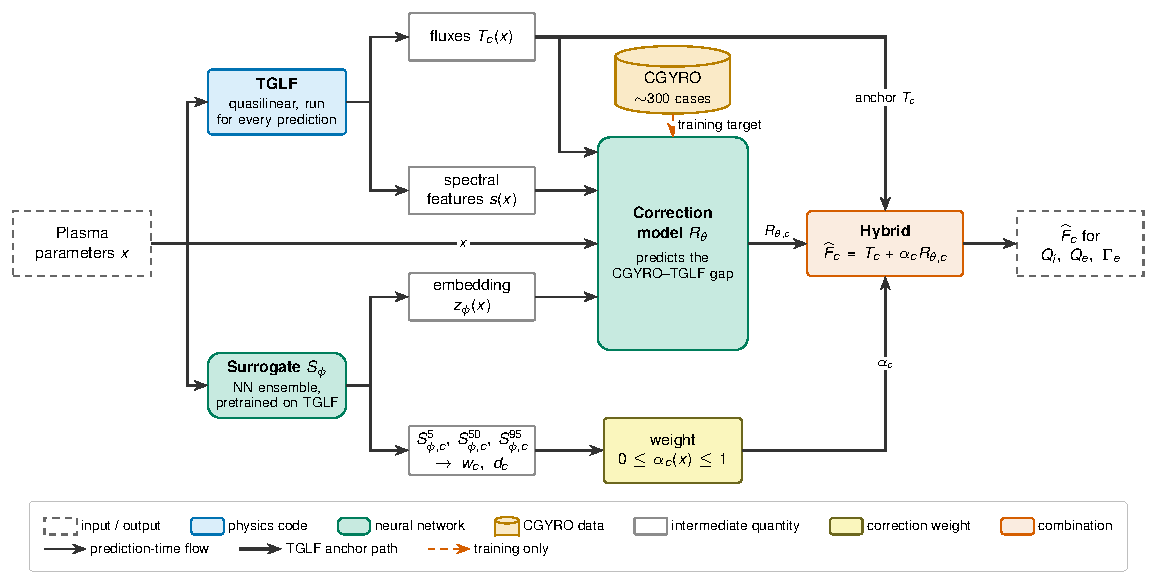
\includegraphics[width=\textwidth]{figures/fig1_hybrid_model.pdf}
      \caption{Hybrid model at prediction time, shown for the additive scale. TGLF fluxes anchor the prediction; $R_\theta$ predicts the CGYRO--TGLF gap from $x$, $T_c(x)$, $s(x)$, and $z_\phi(x)$; and the surrogate's signals $w_c$ and $d_c$ inform the weight $\alpha_c$. CGYRO enters only as the training target.}
      \label{fig:hybrid}
\end{figure}


\begin{table}[H]
      \tablestyle
      \caption{Correction scales.}
      \label{tab:scales}
      \newcommand{\rowstrut}{\rule[-2.4ex]{0pt}{6.2ex}}% equal-height rows that fit the fractions
      \centering
      \begin{tabular}{@{}L{0.9in}L{2.6in}L{1.0in}@{}}
            \toprule
            \textbf{Scale} & \textbf{Hybrid prediction $\widehat F_c$} & \textbf{Channels} \\
            \midrule
            \rowstrut Additive
              & $\displaystyle T_c + \alpha_c\,R_{\theta,c}$
              & $Q_i,\ Q_e,\ \Gamma_e$ \\
            \rowstrut $\operatorname{arcsinh}$
              & $\displaystyle F_0\sinh\!\Big(\operatorname{arcsinh}\frac{T_c}{F_0} + \alpha_c\,R_{\theta,c}\Big)$
              & $Q_i,\ Q_e,\ \Gamma_e$ \\
            \rowstrut Log ratio
              & $\displaystyle T_c\,\exp\!\big(\alpha_c\,R_{\theta,c}\big)$
              & $Q_i,\ Q_e$ \\
            \bottomrule
      \end{tabular}
\end{table}

One scale per channel is selected on the validation split (Table~\ref{tab:design}). The scales weight errors differently:
\begin{itemize}
      \item \textbf{Additive:} a flux offset. It is the simplest to interpret and works for every channel, but the loss is dominated by high-flux cases.
      \item \textbf{Log ratio:} a multiplicative factor, so training targets relative error and weights all flux levels equally. Here $\alpha_c$ acts as an exponent, $\big(e^{R_{\theta,c}}\big)^{\alpha_c}$. It is undefined at zero flux and cannot change sign, so it is used only for $Q_i$ and $Q_e$.
      \item {\boldmath\textbf{$\operatorname{arcsinh}$:}} offset-like for $\lvert F\rvert\ll F_0$ and ratio-like for $\lvert F\rvert\gg F_0$, so it compresses large fluxes and still handles zero and negative values, including $\Gamma_e$. The crossover $F_0$ is tuned.
\end{itemize}

Because the correction is anchored to real TGLF rather than to the surrogate, the residual learned in training is the one corrected at prediction time, and surrogate error does not enter the baseline.

\textbf{Correction weight $\boldsymbol{\alpha_c}$.} The weight $\alpha_c$ sets how much of the correction to apply, from none ($\alpha_c=0$, plain TGLF) to all ($\alpha_c=1$). The aim is to apply the correction only where TGLF is likely to be wrong. Question~2 tests whether two surrogate signals can set $\alpha_c$ case by case:
\begin{itemize}
      \item \textbf{Interval width $\boldsymbol{w_c(x)}$} (Eq.~\ref{eq:width}): wide where TGLF's behavior is hard to learn.
      \item \textbf{Disagreement $\boldsymbol{d_c(x)}$} (Eq.~\ref{eq:disagree}): large where the surrogate fails to match TGLF.
\end{itemize}

Regions that are hard to model may also be where TGLF departs from CGYRO.

\textbf{Cost.} Each hybrid prediction needs one TGLF call (seconds to minutes), against thousands of CPU-hours for a nonlinear CGYRO run. A surrogate-only variant that replaces $T(x)$ with $S_\phi(x)$ needs no physics code and serves as a fast baseline.

\begin{figure}[H]
      \centering
      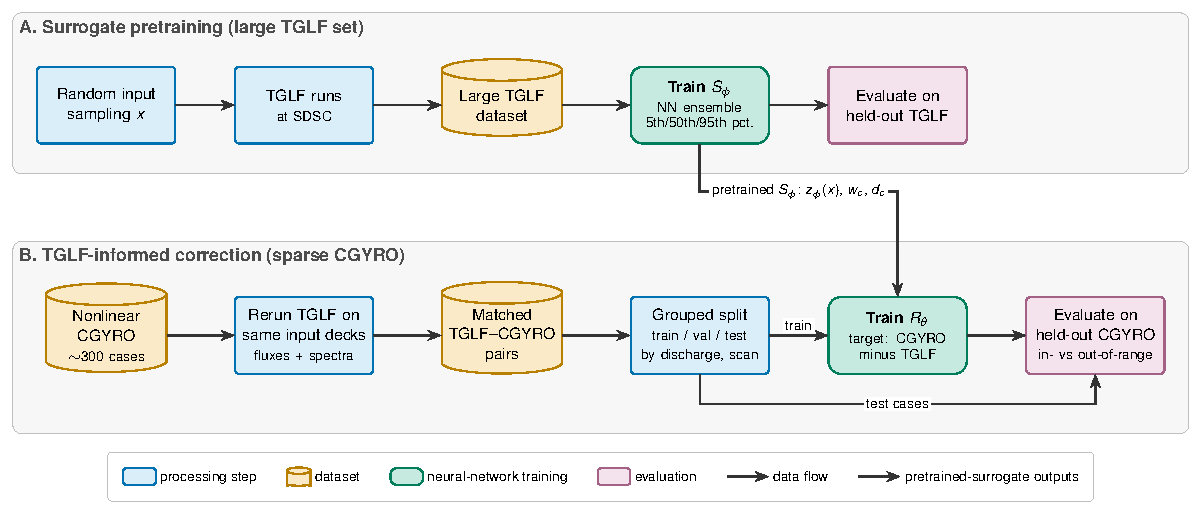
\includegraphics[width=\textwidth]{figures/fig2_data_training.pdf}
      \caption{Data and training pipeline. (A)~The surrogate is pretrained on a large TGLF dataset and supplies $z_\phi(x)$, $w_c$, and $d_c$ to the correction. (B)~The correction is trained on matched TGLF--CGYRO pairs, using splits grouped by discharge and scan, and evaluated on held-out CGYRO cases.}
      \label{fig:pipeline}
\end{figure}


\section{Design choices and experiments}
\label{sec:design}

Experiments run in two stages on fixed, grouped train, validation, and test splits (Section~\ref{sec:eval}):
\begin{itemize}
      \item \textbf{Stage 1, design selection (Table~\ref{tab:design}):} scored on the validation split. Starting from a default configuration (frozen surrogate, hand-picked spectral features, $\operatorname{arcsinh}$ scale, one fixed $\alpha_c$ per channel, ensemble intervals), each experiment changes one choice and keeps the best option.
      \item \textbf{Stage 2, ablations (Table~\ref{tab:ablations}):} the selected configuration is frozen and evaluated on the test split. Each ablation changes one component, so any change in error can be attributed to it.
\end{itemize}

\begin{table}[!tp]
      \tablestyle
      \caption{Stage 1: design choices, selected on the validation split.}
      \label{tab:design}
      \begin{tabular}{@{}B{1.3in}L{3.05in}L{2.2in}@{}}
            \toprule
            Choice & \textbf{Options compared} & \textbf{Notes} \\
            \midrule
            %
            D1. Architecture \q{How big, and how many models?} &
            \opt One shared model vs.\ one model per channel
            \opt Width, weight decay, and ensemble size &
            With about 300 cases, favor regularization and ensembling over depth.
            \rowsep
            %
            D2. Spectral features \q{How are TGLF spectra summarized as $s(x)$?} &
            \opt None
            \opt Hand-picked: peak growth rate per mode type, dominant mode, electron-scale flux fraction, flux-weighted mean $k_y$
            \opt Principal components of the spectra
            \opt Small encoder trained on the large TGLF set &
            Keep the feature count small to limit overfitting.
            \rowsep
            %
            D3. Correction scale \q{In what space is the residual learned?} &
            \opt Additive
            \opt $\operatorname{arcsinh}(F/F_0)$, with a grid over $F_0$
            \opt Log ratio ($Q_i$ and $Q_e$ only) &
            One scale per channel (Table~\ref{tab:scales}). Log ratios need a floor or exclusion at zero flux.
            \rowsep
            %
            D4. Surrogate coupling \q{How much of $S_\phi$ is retrained on CGYRO?} &
            \opt Frozen, with $z_\phi(x)$ as fixed features (default)
            \opt Fine-tune the final layers, jointly with $R_\theta$ &
            Fine-tuning on about 300 cases risks overfitting.
            \rowsep
            %
            D5. Interval method \q{Where does the 5--95\% interval come from?} &
            \opt Spread across an ensemble of correction models
            \opt Direct quantile prediction
            \opt Either, widened by CGYRO time-averaging error &
            Target close to 90\% coverage. TGLF is deterministic and has no interval of its own.
            \\
            \bottomrule
      \end{tabular}
\end{table}

\begin{table}[!tp]
      \tablestyle
      \caption{Stage 2: ablations, reported on the test split.}
      \label{tab:ablations}
      \begin{tabular}{@{}B{1.3in}L{3.05in}L{2.2in}@{}}
            \toprule
            Ablation & \textbf{Variants compared} & \textbf{What it tests} \\
            \midrule
            %
            A1. Baselines \q{Question~1} &
            \opt Uncorrected TGLF ($\alpha_c=0$)
            \opt Pretrained surrogate $S_\phi$ alone
            \opt NN trained on CGYRO from $x$ only, with no TGLF input
            \opt Full hybrid model &
            Whether the correction beats TGLF, and whether anchoring to TGLF beats learning CGYRO from scratch.
            \rowsep
            %
            A2. Information sources \q{Question~4} &
            Inputs to $R_\theta$:
            \opt $x$ and TGLF fluxes $T(x)$
            \opt $+$ spectral features $s(x)$
            \opt $+$ surrogate embedding $z_\phi(x)$
            \opt $+$ both (full model) &
            What each input adds to the correction.
            \rowsep
            %
            A3. Running TGLF \q{Question~4} &
            \opt Hybrid model with $T(x)$
            \opt Surrogate-only variant with $S_\phi(x)$ in place of $T(x)$ &
            What running TGLF adds over a model with no physics code.
            \rowsep
            %
            A4. Uncertainty signals \q{Question~2} &
            \opt Rank correlation of $w_c(x)$ and $d_c(x)$ with the TGLF error $\lvert F^{\mathrm{CGYRO}}_c-T_c\rvert$ &
            Whether the surrogate's uncertainty flags where TGLF departs from CGYRO.
            \rowsep
            %
            A5. Correction weight \q{Question~2} &
            \opt $\alpha_c=0$; one fixed $C$; one fixed $C_c$ per channel
            \opt Learned $\alpha_c(x)$ from $w_c(x)$, $d_c(x)$, distance to the nearest CGYRO case, or ensemble spread, each alone and then combined &
            Whether a case-by-case $\alpha_c$ beats a fixed one. $\alpha_c$ is fit on a validation fold, not on $R_\theta$'s training cases.
            \rowsep
            %
            A6. Amount of CGYRO data \q{Question~3} &
            \opt 25\%, 50\%, 75\%, and 100\% of the training cases, several random draws per size &
            How many cases the correction needs, and whether more runs would help.
            \rowsep
            %
            A7. Transfer \q{Question~1} &
            \opt In-range vs.\ out-of-range test cases (Section~\ref{sec:eval})
            \opt Breakdown by dominant mode &
            Where the correction transfers and where it makes predictions worse.
            \\
            \bottomrule
      \end{tabular}
\end{table}

\section{Evaluation under sparse nonlinear coverage}
\label{sec:eval}

\textbf{Reference data.} Each model is tested against the data it is meant to match:
\begin{itemize}
      \item \textbf{Pretrained surrogate:} held-out TGLF runs. This measures how well it reproduces TGLF and whether the inputs suffice to predict the fluxes.
      \item \textbf{Corrected model:} held-out CGYRO cases. TGLF test cases cannot show its value, since a useful correction should move predictions away from TGLF.
\end{itemize}

\textbf{Metrics.} For each model we report the mean absolute error of the median prediction, and the coverage and average width of the 5--95\% intervals.

\textbf{Splits.} CGYRO test cases are grouped by distance to the nearest CGYRO training case in input space. In-range cases test interpolation; out-of-range cases test transfer. Cases from the same discharge or parameter scan are held out together, so near-duplicates cannot leak between training and test sets. If there are few in-range cases, we report only out-of-range results, with their uncertainty.

% Tables 2 and 3 float, but must appear before this section.
\FloatBarrier
\section{Challenges, quarter plan, and outcome}

\textbf{Challenges.} We expect two main challenges:
\begin{enumerate}
      \item \textbf{Choosing among many design decisions:} the study has many open choices (Tables~\ref{tab:design} and~\ref{tab:ablations}). We must decide which metrics to prioritize when comparing runs, and which proposed runs are worth carrying forward at all.
      \item \textbf{Beating the state of the art:} the correction must achieve higher accuracy than current TGLF saturation rules, including SAT3 \cite{dudding2022} and learned saturation rules such as SAT3-NN \cite{sar2026}.
\end{enumerate}

\begin{table}[H]
      \tablestyle
      \caption{Quarter plan.}
      \label{tab:plan}
      \begin{tabular}{@{}L{0.95in}L{5.78in}@{}}
            \toprule
            \textbf{Period} & \textbf{Milestone} \\
            \midrule
            Winter break & Prepare the TGLF and CGYRO data, and build the initial model and functions: the TGLF surrogate, a basic neural correction, and a final prediction using the additive scale. \\[3pt]
            Weeks 1--2 & Build the remaining functions and test them to make sure runs are valid. Collect initial results and run Stage~1 design selection (Table~\ref{tab:design}) to decide which experiments are not worth pursuing. \\[3pt]
            Weeks 3--5 & Run most of the experiments, including the Stage~2 ablations (Table~\ref{tab:ablations}), repeating each with several random seeds to measure both the accuracy and the precision of the system. \\[3pt]
            Weeks 6--7 & Analyze results: collect the results of all runs, compute correlations, and draw conclusions. \\[3pt]
            Weeks 8--10 & Reserved for writing a paper draft and cleaning up the code so it is reproducible. \\
            \bottomrule
      \end{tabular}
\end{table}

\textbf{Outcome.} The goal is an accurate model of nonlinear CGYRO fluxes that needs only one TGLF call per prediction, reducing the time needed for CGYRO-level predictions by a significant margin.

      {\small
            \begin{thebibliography}{9}
                  \setlength{\itemsep}{2pt}
                  \setlength{\parskip}{0pt}
                  \bibitem{neiser2024}
                  Neiser et al. (2024). Large database validation of TGLF on DIII-D and
                  MAST-U plasmas. \textit{APS Division of Plasma Physics}, conference abstract
                  PP12.00097. \href{https://meetings-archive.aps.org/dpp/2024/pp12/97/}{APS abstract}.
                  \bibitem{sar2026}
                  Sar et al. (2026). A machine learning framework for developing quasilinear
                  saturation rules of turbulent transport from linear gyrokinetic data.
                  Preprint. \href{https://arxiv.org/abs/2604.00462}{arXiv:2604.00462}.
                  \bibitem{cao2026}
                  Cao et al. (2026). TGLF-WINN: data-efficient deep learning surrogate for
                  turbulent transport modeling in fusion. \textit{Nuclear Fusion}.
                  \href{https://doi.org/10.1088/1741-4326/ae72a6}{doi:10.1088/1741-4326/ae72a6}.
                  \bibitem{dudding2024}
                  Dudding, H. (2024). \textit{SAT3 Dataset}, version 1. Zenodo.
                  \url{https://zenodo.org/records/14505760}.
                  \bibitem{dudding2022}
                  Dudding, H. G. et al. (2022). A new quasilinear saturation rule for tokamak
                  turbulence with application to the isotope scaling of transport.
                  Nuclear Fusion 62, 096005.
                  \href{https://doi.org/10.1088/1741-4326/ac7a4d}{doi:10.1088/1741-4326/ac7a4d}.
                  \bibitem{meneghini2017}
                  Meneghini, O. et al. (2017). Self-consistent core-pedestal transport
                  simulations with neural network accelerated models.
                  Nuclear Fusion 57, 086034.
                  \href{https://doi.org/10.1088/1741-4326/aa7776}{doi:10.1088/1741-4326/aa7776}.
                  \bibitem{candy2016}
                  Candy, J., Belli, E. A., and Bravenec, R. V. (2016). A high-accuracy
                  Eulerian gyrokinetic solver for collisional plasmas.
                  \textit{Journal of Computational Physics} 324, 73--93.
                  \href{https://doi.org/10.1016/j.jcp.2016.07.039}{doi:10.1016/j.jcp.2016.07.039}.
                  \bibitem{staebler2007}
                  Staebler, G. M., Kinsey, J. E., and Waltz, R. E. (2007). A theory-based
                  transport model with comprehensive physics.
                  \textit{Physics of Plasmas} 14, 055909.
                  \href{https://doi.org/10.1063/1.2436852}{doi:10.1063/1.2436852}.
            \end{thebibliography}
      }
\end{document}

